\chapter{Reconstruction} % 
\label{sec:reco}

The precise measurement of particles produced in the high energy collisions at the LHC 
is necessary to effectively execute the CMS physics programme. This requires high precision
reconstruction and identification of physics objects in a challenging environment containing
large numbers of different particles with a range of energies. The \alphat analysis 
relies directly on reconstruction of jets and \met for the signal region and on the 
reconstruction of leptons and photons to reject electroweak 
backgrounds and to define control regions.
This requires the use of information from all detector subsystems and state-of-the-art
techniques to allow the reconstruction, selection and calibration of these physics objects.


\section{Detector reconstruction}

The first stage in reconstructing the physics objects is to produce the necessary
input information from the detector subsystems. This information may be tracks
(trajectories) of charged particles or energy measurements from calorimeter depositions. 
Specialist algorithms which suppress backgrounds, mitigate the effects of pileup and provide high resolution energy,
position and/or temporal measurements are used to optimise the precision of the 
measured quantities over a wide range of particle energies and momenta.

\subsection{Track reconstruction}

Charged particle tracks are reconstructed from the hits, considering the efficiency and resolution, 
using the iterative Combinatorial Track Finder (CTF) algorithm. The track reconstruction can be decomposed 
into four logical steps outlined below.

\begin{itemize}
\item Seeds are generated using either triplets of tracker hits or pairs of hits with an additional constraint 
from the beamspot or a pixel vertex. This gives an initial estimate of the trajectory with uncertainty~\cite{tracker_early}.
\item Each seed is propagated outward through the tracker layers while considering the current uncertainty in the trajectory.
In propagating, a uniform magnetic field is assumed as well as no energy loss or multiple Coulomb scattering effects.
The track parameters are updated with the best matching hit on each layer (if any) according to the Kalman filter formalism~\cite{tracker_vertex}.
The search continues until either the boundary of the tracker is reached or no more compatible hits are found. If a minimum number
of valid hits are observed an inwards search is initiated for additional hits~\cite{tracker_early}.
\item It is possible for a single charged particle track to be reconstructed more than once, starting either from different seeds or if
one seed develops into multiple track candidates. If the fraction of shared hits between two track candidates is greater
than 19\% (determined empirically) the track with fewer hits is discarded. If the number of hits is equivalent the track with
 the largest $\chi^2$ is discarded~\cite{tracker_vertex}.
\item After the track candidates are built and cleaned the hits in each candidate are refitted using a Kalman filter and smoother. This 
avoids possible bias from the seeding stage~\cite{tracker_vertex}.
\end{itemize}

The CTF performs six iterations to determine the tracks. Between each iteration any hits that are assigned to tracks in the
previous iteration are removed from the collection. The final track collection is then filtered to remove fake tracks using 
information on the number of hits, the $\chi^2$ and the compatibility of the track originating from a pixel vertex. The momentum 
resolution achieved is 0.7 (5)\% at 1 (1000) \GeV~in the central region~\cite{tracker_early}. Using a dataset of pions and muons from an early run 
at the LHC the tracking efficiency was measured as 98\% for tracks with $\pt > 500\MeV$ and $>99\%$ for tracks with $\pt > 2\GeV$\cite{tracker_eff}.

\subsection{Vertex Reconstruction}

As described in Sec.~\ref{lhc_intro}, the LHC produced an average of 25 simultaneous collisions per bunch crossing
during Run 2. It is essential to identify the Primary Vertex (PV) and the particles originating from it to allow 
particles from additional collisions to be rejected and to identify features such as displaced vertices. The tracks
are initially clustered using a deterministic annealing (DA) algorithm based on the points of closest approach of the 
tracks to the beamspot~\cite{tracker_vertex}. The candidate vertices containing at least two tracks are then
fitted using an adaptive vertex fitter (AVF) to compute the best estimates of vertex parameters~\cite{tracker_avf}. 
Each track in the vertex is assigned a weight between 0 and 1 corresponding to the likelihood that that track
belongs to the vertex. The tracks with weight near 1 are most consistent with the reconstructed vertex while
those that are least consistent have small weights. The number of degrees in the fit, defined as 

\begin{equation}
n_{dof} = -3 + 2 \sum_{i=1}^{\#tracks} wi,
\end{equation}

is an important parameter for distinguishing real proton-proton interactions from misclustered vertices as it is strongly corrected with
the number of tracks compatible with arising from the interaction region~\cite{tracker_vertex}. The vertex
position and resolution determined using the AVF have been 
measured in early LHC data and compared with simulation as shown in Fig~\ref{fig:pvEffRes}.

\begin{figure}[hbt]
  \begin{center} 
   \subfigure[\label{fig:pvEff}]{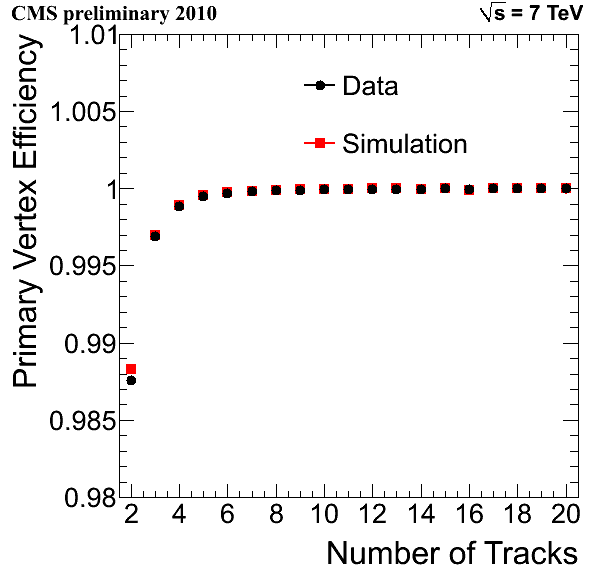
\includegraphics[width=0.5\textwidth]{Figures/detector/pvEff}}~
   \subfigure[\label{fig:pvRes}]{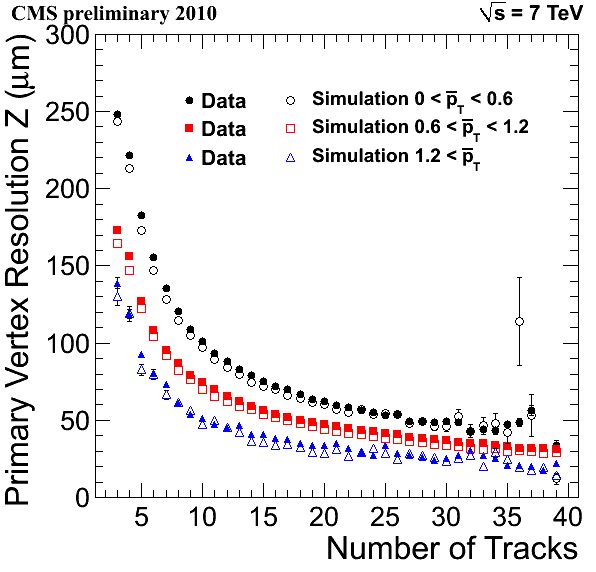
\includegraphics[width=0.5\textwidth]{Figures/detector/pvRes}}
   \caption{(a) Primary Vertex efficiency as a function of the number of associated tracks. (b) Primary Vertex 
   resolution in the z coordinate as a function of the number of associated tracks for three track \pt~scenarios~\cite{tracker_seven}
   \label{fig:pvEffRes} }
  \end{center}
\end{figure}

The vertices are ordered according to the sum of the $p_T^2$ of the tracks associated to each vertex with the 
vertex with the highest $p_T^2$ taken as the primary vertex (PV). The position of the primary vertex can
be used for object identification and control of pile-up. Many CMS analyses, including the one in this 
thesis, make requirements that a good vertex is reconstructed from the tracks satisfying:

\begin{itemize}
\item A minimum number of degrees of freedom: $n_{dof} > 4$.
\item The collision to occur with $|z| < 24cm$ such that the primary vertex is near the 
interaction point in the longitudinal direction.
\item The collision to occur within a radial distance of $|d_{xy}| < 24cm$ from the beamline.
\end{itemize}

\subsection{Calorimeter reconstruction}

The calorimeters reconstruct the energies of incident particles from deposits made in the 
various subsystems. These deposits must be clustered and the measurement calibrated to provide 
details of the energy, position and timing of the incident particle.
For neutral particles the calorimeter subsystems provide the only measurement of
the particle properties. For charged particles the measurement complements that
from the tracker and provides necessary redundancy in the case of track
misreconstruction.

The ECAL crystals are calibrated with both absolute and relative calibrations. Nine EB superclusters
and 500 EE crystals are calibrated using high energy electron beams to achieve a 
resolution of 0.5\% (1\%) for the EB (EE) components~\cite{ecal_calib}. 
The remainder undergo relative intercalibrations to achieve a resolution of 1.4\%-1.8\% ($\sim5\%$) 
for the EB (EE) components. During LHC runs the response of the crystals changes due to 
radiation induced crystal-lattice defects which absorb the scintillation light. 
The crystal transparency is monitored to allow the impact on energy measurements to
be assessed and corrected~\cite{ecal_calib}. 

The HCAL components undergo a similar calibration to the ECAL crystals. Firstly a subset of the 
components are calibrated with a 50 \GeV~pion beam which is then extended to the remainder of the 
subsystem using a Co source~\cite{hcal_beam}. Additional corrections
for the HCAL component are derived during LHC running~\cite{hcal_calib}.

The reconstruction of the energy at the HCAL and ECAL relies on recording the amplified 
light pulses from the photodiodes over a 25ns time sample. When operating with 25ns bunch 
spacing, particle energies from previous or following bunch crossings can be integrated
into this sample, biasing the energy measurement. This effect is correcting by using a 
dedicated reconstruction that removes the contributions from such Out Of Time Pileup 
(OOTPU)~\cite{hcal_timing,ecal_timing}. The 25ns sample is fitted including three pulse 
shape templates with variable amplitude and arrival times with the central pulse corresponding 
to the triggered event. The timing distribution for the ECAL hits above 1~\GeV, which is derived 
independently from the energy measurement, is shown in Figure~\ref{fig:timing_barrel_linear} 
showing the effective rejection of contributions from OOTPU.

\begin{figure}
\centering
    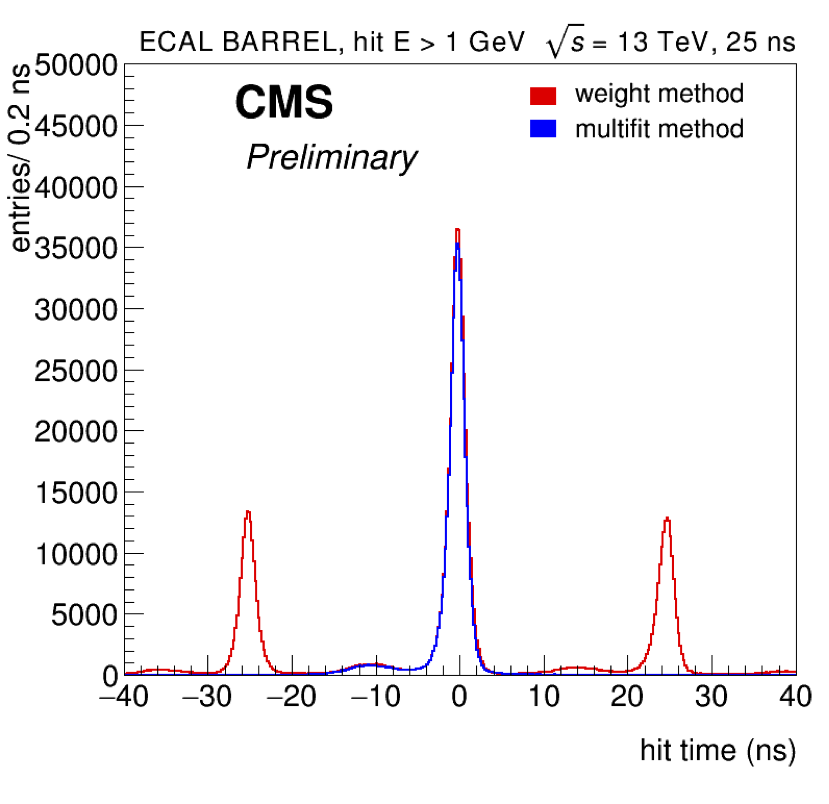
\includegraphics[width=0.8\textwidth]{./Figures/reconstruction/timing_barrel_linear.png}
  \caption{Timing distribution of the hits in the ECAL barrel with a reconstructed energy above 1\GeV~\cite{ecal_timing}.}
  \label{fig:timing_barrel_linear}
\end{figure}

\section{Physics object reconstruction}

The reconstructed tracks and calorimeters form the inputs to the reconstruction of the particles and 
jets that form the basis of the final selection of many analyses, including the analysis described 
in the thesis, referred to as physics objects. These are reconstructed using a combination of
dedicated local reconstruction algorithms as well as the global event Particle
Flow algorithm, described in Section~\ref{sec:particle_flow}.
In addition, several WPs of selection criteria are defined for each physics object 
which provide a range of efficiencies and corresponding proportion of false positives. 

\subsection{Electron and photon reconstruction}
\label{sec:ele_pho_reco}

Photons and electrons interact similarly within the ECAL and so these objects 
follow similar reconstruction techniques. Electrons are reconstructed by matching 
information in the tracker and ECAL using two complementary techniques, an ECAL driven 
reconstruction described in this section (identical, aside from tracking
requirements, to the photon reconstruction) and a tracker-driven reconstruction performed with
the PF algorithm (see Section~\ref{sec:particle_flow}) which is optimal for low \pt~electrons. 

In the ECAL, both electron and photon candidates are formed by clustering energy deposits
from electromagnetic showers. Around 50\% of the photons convert into an electron-positron 
pair in the material proceeding the calorimeter leaving an energy deposit that is widely 
spread in $\eta$ and $\phi$~\cite{electron_photon_reco}.  For unconverted photons the 
deposits are fairly localised in $\eta$ and $\phi$. Electrons radiate
bremsstrahlung along their trajectories due to the presence of the magnetic field and 
lose $33\%$ of their energy on average in the central region 
and up to $86\%$ at $|\eta| = 1.4$. Their energy deposits are widely spread in $\phi$ but narrow in $\eta$. 
The hybrid (multi) clustering algorithm exploits this characteristic to
reconstruct high energy electrons and photons in the barrel (endcap). The hybrid algorithm
uses a seed crystal and clusters up to ten \emph{dominoes} of $1\times3$ or $1\times5$ ($\phi\times\eta$) within 
$\Delta\phi < 0.3$ from the seed. Any domino with an energy under $100\MeV$ is discarded. The dominoes
are themselves clustered in $\phi$ provided each disconnected subcluster has a seed 
domino of energy $>350\MeV$. The combination of these subclusters is referred 
to as a supercluster. The reconstruction in the endcap follows a similar procedure 
using $5\times5$ grids of crystals. 

Superclusters which can be associated to tracks originating from the primary vertex are reconstructed as electrons.
As electrons lose energy through the non-Gaussian bremsstrahlung process the Kalman filter is inappropriate and
so the specialist track reconstruction Gaussian Sum Filter (GSF) algorithm is used. This allows the total energy of
electrons to be reconstructed including the component lost through bremsstrahlung. The photons are identified 
through inverting the track matching criteria of the supercluster. In the endcaps, additional information
is used from the preshower when reconstructing the energy.

Additional selections are applied on all reconstructed electrons and photons to suppress backgrounds.
For electrons these are mainly composed of misreconstructed jets, secondary electrons from photon
conversions and semi-leptonic decays of heavy quarks. As electrons are mainly contained within 
the ECAL, a requirement on the ratio of energies in the ECAL and HCAL provides a strong veto of hadronic
backgrounds. In addition, requirements are made on the matching track \emph{impact
parameters} such that the transverse distance from the primary vertex is $d_{xy} < 0.0261$ ($d_{xy} < 0.118$) 
and the longitudinal distance is $d_z < 0.041$ ($d_z < 0.822$) for the barrel (endcap). 
Several variables that rely on the shower shape and cluster width are used to
reject fakes, including $\sigma_{i\eta i\eta}$ (the second moment of the log-weighted
distribution of crystal energies calculated in the $5\times5$ matrix around the
most energetic crystal). The value of $\sigma_{i\eta i\eta}$ allows background
processes to be rejected as its value is larger on average for neutral meson decay to two collimated photons.

\subsection{Muon reconstruction}
\label{sec:muon_reco}

As muons are MIPs they leaving minimal energy deposits in the calorimetry
subsystems and travel through the entire detector. The muons are therefore reconstructed using a 
combination of the inner tracker and muon systems. Two algorithms are used to 
give complementary efficiency across the momentum spectrum, the 'the outside-in' 
global muon algorithm and 'the inside-out' tracker muon algorithm~\cite{muon_reco}.

The outside-in algorithm begins with muon tracks and for each attempts to
identify a tracker match. Hits in muon chambers are used to define standalone-muon tracks. 
These are matched with tracker tracks by comparing parameters of the two tracks propagated 
onto a common surface. The hits from both systems are then combined and a global muon fit 
is performed using a Kalman filter. For muon tracks the momentum resolution is significantly improved by 
the global fit over a tracker only fit for $p_T < 200\GeV$~\cite{CMS,muon_reco_cosmic}. 

The inside-out algorithm selects all tracks satisfying $p_T > 0.5\GeV$ and $p > 2.5\GeV$. These are then 
extrapolated to the muon system taking into account effects from the magnetic field, multiple Coulomb scatting
in the detector material and the average expected energy loses. If at least one muon segment matches 
the extrapolated track, the track qualifies as a tracker muon. Tracker muon reconstruction is more efficient
than global muon reconstruction for low momenta of $\sim p< 5\GeV$. This is due
to only requiring a hit in one segment of the muon system while global muon reconstruction is 
more efficient for higher energy muons which are likely to pass through several muon stations~\cite{muon_reco}.

In order to ensure the muons are prompt (produced in by the hard process such as vector boson decay) rather
than non-prompt (produced from the in-flight decays of hadrons, taus or heavy quarks) and to reject fakes
caused by the punch through of hadronic particles, additional selections are made. These include quality
selection on the $\chi^2$ of the muon track, a minimum number of valid hits as well as requirements
on the impact parameters $d_{xy} < 0.05 cm$ and $d_{z} < 0.1 cm$ aimed at ensuring prompt muons.

Muons must be reconstructed through either the global or tracker muon algorithm. In combination, and
including additional selections, these provide an efficiency of $>95\%$ for reconstructing a muon 
with \pt~larger than a few \GeV~over the full $\eta$ range covered by the
muon system and a fake rate from hadrons of $<1\%$~\cite{muon_reco}.

\section{Particle Flow}
\label{sec:particle_flow}
The particle flow (PF) algorithm combines the inputs from dedicated track reconstruction and calorimeter clustering
algorithms using all detector subsystems to identify and reconstruct all stable particles in the event.
Despite hundreds of different particle species being produced by collisions at the LHC only a small fraction
have sufficient lifetimes and interactions with the detector to be directly measured. The predominant species
measured by the CMS detector are: $\gamma$, $e^{\pm}$, $\mu^{\pm}$, $\pi^{\pm}$, $K^{\pm}$, $p^{\pm}$, $K^{0}$
and $n$, classified by the PF algorithm into five categories of photons, electrons, muons, charged hadrons and neutral hadrons. 
The identification and measurement of the properties of these particles is optimised by taking advantage of the complementarity of 
different subsystems in various kinematic regimes and geometries over the performance achievable with 
any one subsystem alone. The output list of the individual particles is similar to that provided
when generating Monte Carlo events. This can then be used to as an input for further reconstruction processes
such as building jets, determining \met~, determining jets originating from bottom quarks (b tag) and quantifying
charged lepton isolation. The algorithm is described fully in~\cite{pf_proc,pf_pas}.

Effective track reconstruction forms the core of the PF algorithm. The CMS detector, with a strong magnetic field
and large silicon tracker, is highly capable of the efficient track
reconstruction required. In addition, the high granularity ECAL allows effective separation of photons from 
charged particles, even inside jets of several hundred \GeV, and the entire calorimetry system 
is included within the solenoid, allowing an uninterrupted measurement 
of the particle energy flow.

The PF algorithm utilises a specific clustering algorithm for calorimeter deposits which is performed separately 
in each calorimeter sub-detector. First, cluster seeds are identified as local cell maxima over a threshold energy.
Second, these are grown into topological clusters by aggregating any cells with at least one side in common with
a cell already in the cluster and with an energy above a given, detector
subsystem dependant, threshold. Finally, the total energy in each topological cluster
is shared between all encompassed seed clusters according to the cell-cluster distance to 
form a PF cluster for each seed. Along with reconstructed tracks, these PF clusters form the inputs 
required to build PF candidates.

The PF reconstruction uses a link algorithm to iteratively check compatibility of charged particle tracks 
and/or calorimetry clusters and/or muon tracks. These elements must be connected while avoiding any double counting. 
The link algorithm is performed on every pair of elements in the event and defines a distance between them
that quantities the quality of the link. This is used to produce blocks of elements linked directly 
or indirectly. The blocks are constructed depending on the subsystems being linked as described below:

\begin{itemize}
\item A link between a charged particle track and calorimeter deposit is made by extrapolating the last measured
hit in the tracker through the calorimetry systems. The track is linked to a cluster if the calorimeter position
is within the cluster boundaries. The link distance is defined as the distance in the ($\eta,\phi$) plane between
the extrapolated track position and cluster position.
\item Clusters caused by bremsstrahlung photons emitted by electrons are associated to the track by extrapolating
the tangents to the track from the intersection points of the track with tracker layers to the ECAL. The distance measure
is the same as defined above.
\item Calorimeter clusters are linked between HCAL and ECAL or between ECAL and PS clusters by establishing whether
the cluster in the more granular calorimeter is within that of the less granular. The link distance is defined
as the distance in the ($\eta,\phi$) plane between the cluster positions.
\item Charged particles tracks are associated with muon tracks following the global muon algorithm defined in 
Section~\ref{sec:muon_reco}. In this case the $\chi^2$ of the global fit defines the link distance.
\end{itemize}

With the blocks defined, the algorithm for reconstruction and identification of the set of particles from each
block, which forms a global description of the event, proceeds as follows:

\begin{itemize}
\item First, each global muon is defined as a PF muon if its combined momentum is compatible with the momentum 
from the tracker only within three standard deviations. The track is removed from the block and expected energy depositions
along the path of the muon in the calorimeters are subtracted (measured with
cosmic ray muons to be 3 \GeV~and 0.5 \GeV~respectively for the ECAL and HCAL).
\item Electrons are then identified. Tracks are pre-identified as electron tracks based on their 
characteristics within the tracker. Such tracks are refitted with a Gaussian-Sum Filter and extrapolated to the ECAL. 
Several tracking and calorimetric variables are then used to perform a final identification of PF electrons. The track
and ECAL clusters (including those from bremsstrahlung) are removed from the block.
\item The remaining tracks undergo additional quality criteria and are connected to ECAL and HCAL clusters. 
If calorimetric deposits are linked with a track a PF charged hadron is identified. 
\item The detection of neutral particles in addition to the PF charged hadron 
relies on a comparison of the momentum of the tracks and the calibrated energy in the calorimeters. 
The momentum and energy are calculated from the track momentum under a charged pion hypothesis. 
If the calibrated calorimetric energy is significantly in excess of this energy, considering
the calorimetric resolution, a PF photon and possibly a neutral hadron are also identified. 
If the energy excess is larger than the total ECAL energy, a PF photon is created with the ECAL energy and a 
PF neutral hadron is created taking its energy as the remainder of the excess. 
Otherwise, only a PF photon is created with the energy of the excess.
\item Any remaining ECAL and HCAL clusters give rise to PF photons and PF neutral hadrons respectively.
\end{itemize}

\subsection{Pileup estimation}

In reconstructing the hard process it is important to remove contributions from additional
vertices. The PF objects can be used to identify 
charged hadrons which do not originate from the primary vertex. However, the vertex 
for neutral particles cannot be determined. Instead, the ratio of neutral and 
charged particles can be measured in simulation and a correction factor determined.
This is necessary as neutral particles compose $\sim 50\%$ of the pileup in the barrel.
An additional form of pileup subtraction relies on an estimate of the local energy density 
of pileup, $\rho$, which can then be used to correct physics objects covering an area,
A, as

\begin{equation}
p_T^{\text{corr}} = p_T^{\text{raw}} - \rho \cdot A,
\end{equation}

where the values for $\rho$ are determined by partitioning the detector into a square grid of spacing
0.55 and calculating the median energy of the energy density of all PF candidates within each cell (grid $\rho$)~\cite{fastjet,jet_area}.
This effective area (EA) correction mitigates the contributions of both charged and neutral 
pileup particles.

\subsection{Isolation}

The level of hadronic activity around a lepton provides an effective method to distinguish between prompt and non-prompt leptons.
This is measured by the isolation of the lepton, defined by the fraction of energy
in a cone around the lepton to the energy carried by the lepton itself. For the
CMS collaboration, the standard method of measuring isolation during Run 2 
is PF isolation, $I_{PF}^{rel}$, defined within a cone of radius $\Delta R$ as 

\begin{equation}
I_{PF}^{rel} = \frac{1}{p_T^{l}}\left[ \sum_{PF_{PV}}p_T^{CH} +  \sum_{PF}p_T^{NH} +  \sum_{PF}p_T^{\gamma} -  \sum_{PU}p_T^{\text{Neutral}}\right]
\end{equation}

where $p_T^{l}$,$p_T^{CH}$,$p_T^{NH}$,$p_T^{\gamma}$ are the momenta of the lepton, charged hadrons, neutral hadrons and photon respectively.
A subtraction of the neutral pileup must be made as neutral particles cannot be associated with the PV. The $\Delta \beta$ correction
and Effective Area correction are two methods used by CMS to estimate and correct for the neutral pileup contribution. The delta $\Delta \beta$
correction estimates the energy from the neutral hadrons from the charged hadron component, based on simulation, as

\begin{equation}
\sum_{PU}p_T^{\text{Neutral}} = \frac{1}{2} \sum_{PF_{PU}}p_T^{CH}
\end{equation}

while the effective area corrects the expected neutral pileup energy based on the footprint of the particle, $A_{eff}$ and the grid pileup
energy density computed from neutral particles, $\rho_{grid}^{\text{Neutral}}$

\begin{equation}
\sum_{PU}p_T^{\text{Neutral}} = \rho_{grid}^{\text{Neutral}}\cdot A_{eff}.
\end{equation}

the cone size may be fixed (relative isolation) or dependant on the \pt~of the particle (mini-isolation). The use of mini-isolation
accounts for the increasing collinearity of the hadronic decays of boosted particles. 

\subsection{Isolated tracks}

Unreconstructed prompt leptons form a large background for hadronic searches.
Such \emph{lost leptons} can be caused by both acceptance effects and by misreconstruction of 
processes including $e^{-}$, $\mu^{-}$ decays and hadronic decays of $\tau$ leptons. 
Typically, even if not associated to the lepton, the lepton track will still be
reconstructed. Prompt leptons also tend to be isolated and so the background
from misreconstructed leptons can be mitigated by vetoing of high
energy isolated charged tracks. Isolated tracks are defined from PF candidates associated with the PV and 
which pass track quality selection but are not identified as leptons.

\section{Jet reconstruction} 
\label{sec:jet_reco}
As the LHC is a hadron collider, most events will involve the production of quarks and gluons. As discussed in
Section ?? these strongly interacting particles hadronise into collimated jets of particles. As described 
in the following section, the properties of the original parton which originated the
jet can be reconstructed by combining all of the particles forming the jet. In order for the properties of the jet to be theoretically tractable the
reconstruction algorithm has to satisfy the requirements of infrared safety, insensitive to the addition of 
soft particles, and collinear safety, insensitive to collinear splitting of particles.

\subsection{Jet clustering}

To achieve infrared collinear safety, CMS uses a sequential recombination algorithm~\cite{antikt}. The input clusters can represent
the momenta of particles, calorimeter energy deposits or previously clustered
4-vectors. These algorithm define inter-jet distances,

\begin{equation}
d_{ij} = min\left[p^r_{T_i},p^r_{T_j}\right]\left(\frac{\Delta R_{ij}}{R}\right)^2,
\end{equation}

between each pair of clusters i and j, as well as beam-jet distances, 

\begin{equation}
d_{iB} = p^r_{T_i}
\end{equation}

where the $r$ parameter depends on the specific algorithm used, R determines the maximum distance
for clustering pairs and $p_{T_i}$ is the transverse momentum of the cluster. The algorithm then proceeds
as follows:
\begin{itemize}
\item Calculate and rank all the distances, $d_{ij}$ and $d_{iB}$ for all clusters in the event
\item If the smallest distance is an inter-jet distance combine clusters i and j into a new cluster and recalculate distances
\item If the smallest distance is a beam-jet cluster i is considered to be a final state jet and is removed from the event. Distances 
are then recalculated.
\end{itemize}

These steps are repeated until no clusters remain. The algorithm used for the analysis in this thesis (and for most CMS analyses) is 
the anti-$k_T$ algorithm for which $r=2$. The size of the jets is $R=0.4$ which optimises the balance between capturing all particles
associated with a jet and resilience against pileup. CMS uses jets with inputs from PF candidates (PF jets) and calorimeter deposits (calo jets)
clustered using the \FASTJET~package~\cite{fastjet}. PF jets allow improved resolution with respect to calo jets due to the significant position and energy resolution 
enhancement possible with use of the tracker. PF jets are therefore used in offline analysis while calo jets are used only in HLT reconstruction
where latency restrictions forbid the formation of the PF candidates. 

To reject jets which are badly reconstructed or originate from detector noise, additional selections are made. These include at least
two PF candidates, the fraction of energy from neutral hadrons and photons < 99\%,  charged hadron fraction > 0 and charged particle multiplicity > 0.
The rate of fake jets is reduced by 84\% while maintaining $> 99\%$ efficiency for jets from quarks and gluons.

\subsection{Jet energy corrections}

The energy of the clustered jets will not conform to the true partonic energy but instead is approximately Gaussian distributed around this value.
This is due to variation in response in different sections of the detector, at worst, losses in uninstrumented sections of the detector, as well as 
random fluctuations in the particle composition during hadronisation. To recover the true value Jet Energy Corrections (JECs) are applied using the functional
form~\cite{jec}

\begin{equation}
\label{equ:jec}
  p_{\mu}^{\rm{cor}}=C_{\rm{offset}}\left(\pt^{\rm{raw}}\right)\cdot
  C_{\rm{rel}}\left(\eta\right)\cdot C_{\rm{abs}}\left(\pt'\right)\cdot
  C_{\rm{res}}\left(\pt'',\eta\right)\cdot p_{\mu}^{\rm{raw}}.
\end{equation}

where $C_{offset}$, $C_{rel}$, $C_{abs}$ and $C_{res}$ represent offset,
relative, absolute and residual corrections respectively, 
 ($p_{\mu}^{raw}$) $p_{\mu}^{corr}$ is the (uncorrected) corrected jet 4-momentum, $p'_T$ is the \pt~after the 
 offset and relative corrections and  $p'_T$ is the $p''_T$ after
all corrections except the residual. The corrections are described in more detail below~\cite{jec2}:

\begin{itemize}
\item The $C_{offset}$ is the first step in the chain. Its purpose is to remove
energy contributions not associated with the hard scattering the originate from sources
such as noise and pileup. The pileup contributions are removed using Charged
Hadron Subtraction (CHS), where PF candidates not associated to the PV
are removed before clustering, and the jet area method. The jet area method removes neutral component 
of pileup from the jets by subtracting $\rho \cdot A_j$
from the $p^{raw}_T$, where $A_j$ is the active area of the jet and $\rho$ 
is the average pileup energy density, determined from the median energy of PF candidates
across the detector. 
\item The $C_{rel}$ is used to make the energy response uniform in $\eta$ for all jets using MC truth corrections derived from QCD dijet events.
\item The $C_{abs}$ is used to correct the energy response as a function of jet \pt~. This is done using \zj~and \gj~events as for
these processes the boson \pt~is well known which can be used to balance the \pt~of the reconstructed jet.
\item The $C_{res}$ is used to correct residual differences between the responses in both \pt~and $\eta$ for data and MC and applied in data only.
\end{itemize}

Each correction has associated systematic and statistical uncertainties. These are added in quadrature to define the overall jet energy uncertainty. The 
overall uncertainty is shown in Fig~\ref{fig:jec_unc}.

\begin{figure}
\centering
    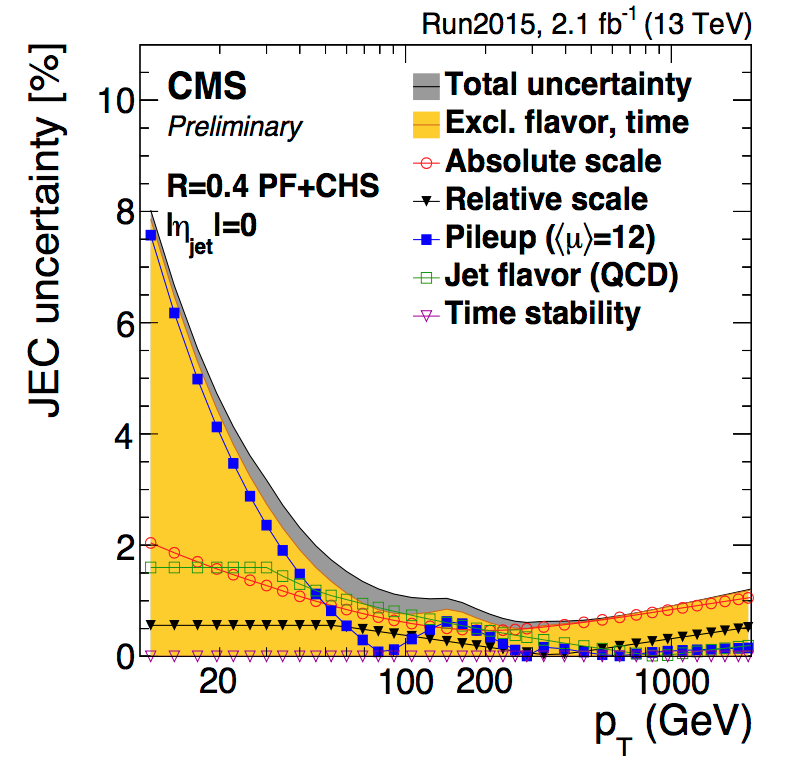
\includegraphics[width=0.8\textwidth]{./Figures/reconstruction/jec_unc.png}
  \caption{\label{fig:jec_unc} The overall uncertainty in the corrections applied to MC from Equation~\ref{equ:jec} shown in the orange solid curve. The pileup uncertainty dominates
for $\pt < 50\GeV$ while for higher values of \pt~the absolute and relative scale dominate~\cite{jec_fig}.}
\end{figure}

\subsection{B tagging}
\label{sec:btag}
For Run 2 the Combined Secondary Vertex version 2 (CSVv2) algorithm is used to tag jets as originating
from b quarks. The algorithm exploits the long lifetime of the b hadron, the secondary vertex of its decay
and the possible presence of a muon or electron (produced in $\sim 20\%$ of the b hadron decays). The 
input variables are combined with a neural net and the secondary vertex
information is obtained using the Inclusive Vertex Finder (IVF) algorithm~\cite{csv_pas}.

The dominant backgrounds for tagging b quarks are jets originating from c quarks and to a lesser extent
jets from lighter quarks and gluons. The distribution of the CSVv2 discriminator is shown for PF Jets
using $13\TeV$~data and simulation in Figure~\ref{fig:csv_fig}. The value of the discriminator
used in the $\alphat$ analysis is 0.89 corresponding to an efficiency of $\sim67\%$ CHECK THIS and 
a mistag rate of $\sim 1\%$ for light quarks ($u$, $d$ and $s$ quarks) and gluons and a mistag rate of $\sim 10\%$ for
charm quarks. The difference in efficiency and mistag rates in data and simulation is measured 
for a range of jet energies to provide scale factors to correct the simulation. In the
Run 2 dataset, these scale factors were around $0.94$ and $\sim1.1-1.3$ (depending on \pt) for the b-tag and mistag SFs 
respectively~\cite{csv_fig}.

\begin{figure}
\centering
    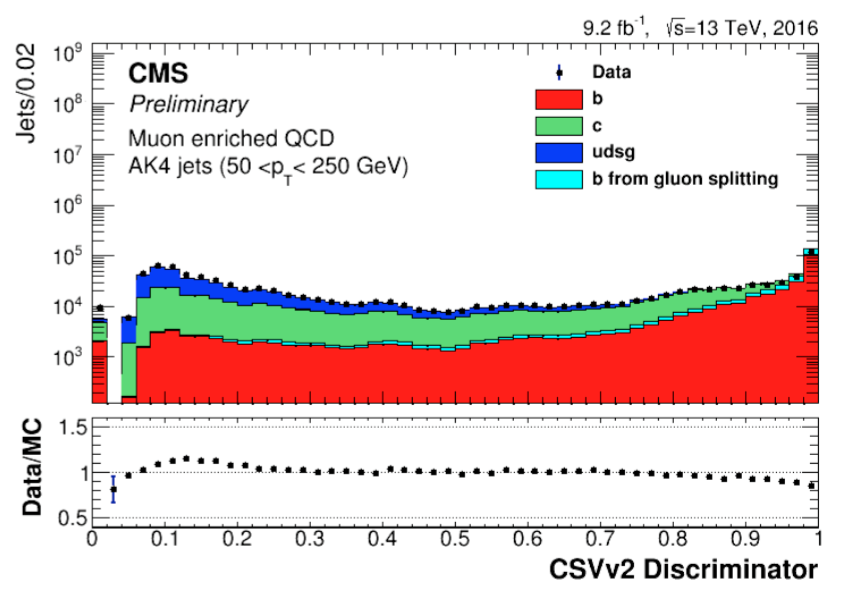
\includegraphics[width=0.8\textwidth]{./Figures/reconstruction/csv_fig.png}
  \caption{\label{fig:csv_fig} Distribution of the CSVv2 discriminator for ak4 jets 
in a muon enriched jet sample (right). The markers correspond to the data. 
The stacked, coloured histograms indicate the contributions of the different 
jet flavours in the simulation~\cite{csv_fig}}
\end{figure}

\subsection{Cross cleaning}

The lepton and jet reconstruction algorithms are run independently and so the same detector
signals may be reconstructed as different physics objects. To avoid this double
counting, a cross cleaning is performed. Any reconstructed jets within $\Delta R < 0.4$ 
of an isolated lepton are removed.

\subsection{Energy sums}
\label{sec:energy_sums_reco}
Energy sums are vital for hadronic searches for new physics such as the $\alphat$~search. The typical high
mass scale of BSM models causes large quantities of energy to be transferred to particles in the final
state. This energy is shared between both visible and invisible particles leading to large total and missing energy
which can be measured by CMS. These signatures provide a crucial separation from the QCD background, typically at
a lower energy scale. The CMS detector is ideally suited to measuring these signatures due to its hermetic design
allowing optimal acceptance for all observable particles in the final state.

To measure the energy scale of the parent process in the event two variables are commonly used. 
These are the total transverse energy, $E_\text{T}$, which is computed as the scalar sum of the transverse 
energies of all reconstructed PF candidates in the event and the total hadronic
transverse energy, \scalht, which is computed as the scalar sum of the transverse energies of all calibrated reconstructed jets:

\begin{equation}
E_\text{T} = \sum |\vec{p}_T^{\text{PF}}| && \scalht = \sum |\vec{p}_\text{T}^{j}|.
\end{equation}

Missing energy in the final state can be caused by BSM phenomena such as the LSP of R-parity conserving SUSY or 
DM particles predicted by generic models of Dark Matter as well as standard
model processes such as neutrinos from vector boson decay. This quantity is reconstructed indirectly from the observed particles in the final state by exploiting
momentum conservation in the transverse plane. Two variables are used in the
\alphat~analysis: the missing transverse momentum, 
\metvec, which is defined as the negative vector sum of the transverse momenta
of all PF candidates and has magnitude \met,
as well as the hadronic missing transverse momentum, \mhtvec, which is defined as the negative vector sum of the
transverse momenta of all calibrated reconstructed jets and has magnitude \mht:

\begin{equation}
\metvec = -\sum \vec{p}_T^{PF} && H_T = -\sum \vec{p}_T^{j}.
\end{equation}

In addition, calorimeter-\metvec, defined as the negative transverse vector sum of the calorimeter deposits, is used 
for the HLT as the PF candidates cannot be reconstructed within latency constraints. The \metvec~is used offline
as the performance is substantially improved by including tracker information~\cite{pf_pas}. 

As a measure of the momentum imbalance, \metvec~can be biased due to effects including 
minimum energy thresholds in the calorimeters, tracker inefficiencies and non=linearities
in calorimeter response. This bias is reduced by correcting the \pt~of CHS corrected PF jets 
using the JECs and propagating the correction to the \metvec~as

\begin{equation}
\vec{E}_\text{T}^{\rm misscorr} = \metvec - \sum_{j}(\vec{p}^{\text{corr},j}_T -
\vec{p}_T^{j}).
\end{equation}

This `type-1' correction~\cite{met_fig}~uses all corrected jets with $\pt > 15\GeV$ with less than 0.9 of their energy deposited in the ECAL.
The 4-momenta of any muons found in jets are subtracted when performing the correction and added back to the corrected object.
Figure~\ref{fig:met_fig} shows excellent agreement between simulation and data
in reconstructing the \met~with 13\TeV~Run 2 data.

\begin{figure}
\centering
    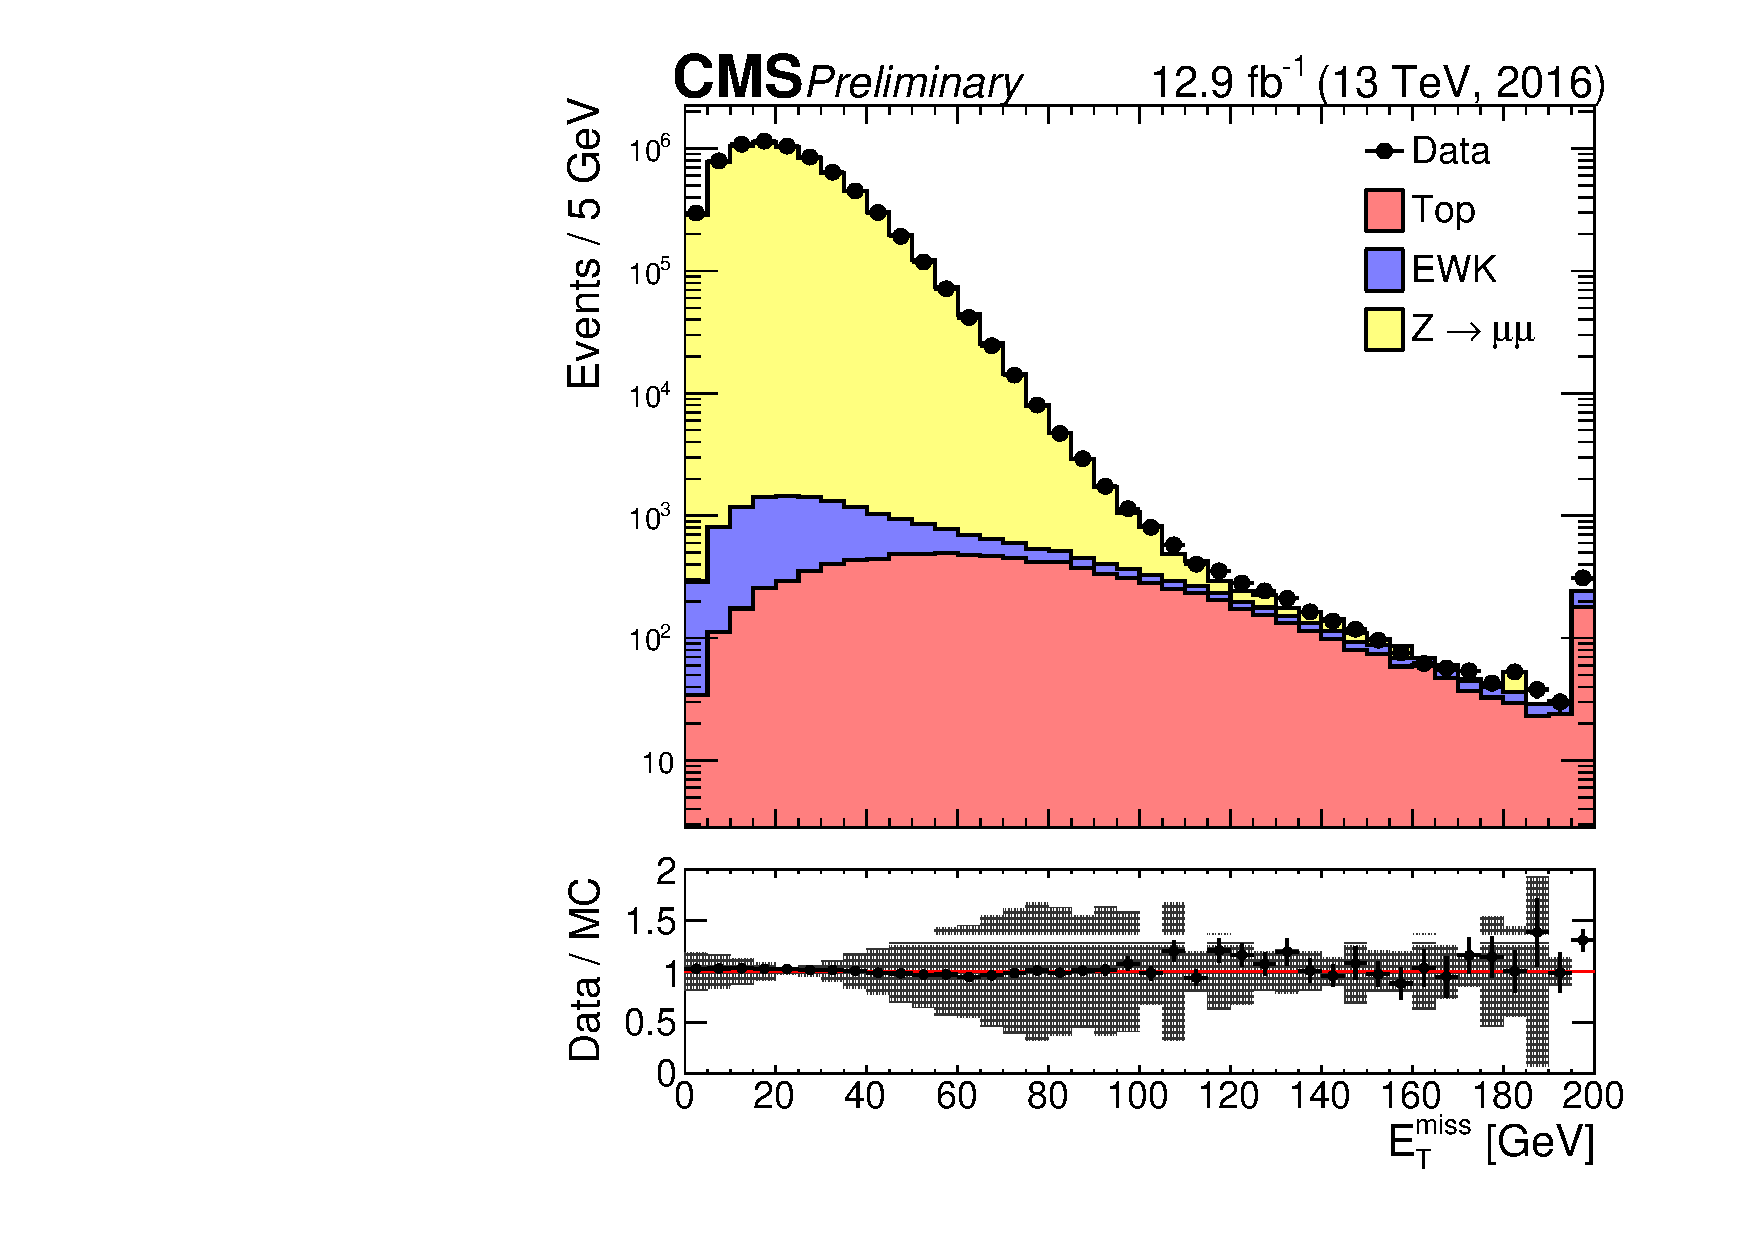
\includegraphics[width=0.8\textwidth]{./Figures/reconstruction/met_fig.pdf}
  \caption{Distribution of \met~in \zmumu candidate events. The markers show the data while the filled coloured histograms
  show the breakdown in difference processes for the simulation. The lower panel shows the data/MC ratio including
  both statistical and systematic uncertainties~\cite{met_fig}. \label{fig:met_fig} 
}
\end{figure}

\section{Physics objects for the \alphat~analysis}

The \alphat~analysis makes use of the reconstruction algorithms described above
to identify and reconstruct physics objects. The analysis uses a hadronic signal 
region with jets and large~\met as well as several signal depleted regions used to predict the
backgrounds in the signal region, the hadronic, \gj, \mj and \mmj control regions defined in 
Section~\ref{sec:cr-sel}. This section describes the definition of the 
physics objects used for the \alphat~analysis.

\label{sec:phys-obj}
\subsection{Jets}

The jet collection is defined by PF jets (clustered from PF candidates) as defined in Section~\ref{sec:jet_reco} with
$\Delta R = 0.4$. The jets are corrected for pileup contributions using CHS and jet area corrections. Additional cleaning cuts are then applied
on the jet constituents as summarised in Table~\ref{tab:loose-jet-id}. These requirements are necessary to reject fake jets. The charged hadron
fraction cut of $> 0.1$ additionally rejects jets reconstructed from beam halo interactions.

A threshold of jet $\pt > 40 \GeV$ is required for jets used in the analysis. As supersymmetric models tend to produce
relatively hard jets this provides a good efficiency while effectively rejecting QCD backgrounds. Jets in the signal 
region must satisfy the pseudorapidity requirement $\etaabs < 2.4$. The presence of any forward jets with $\etaabs > 2.4$
is used as a cleaning veto as described in Section~\ref{sec:fwd_jet_veto}. Additionally, the leading jet in the 
event must satisfy $\pt > 100\GeV$. 
\begin{table}[ht!]
  \caption{Jet identification requirements. \label{tab:loose-jet-id}}
  \centering
  \begin{tabular}{ ccc }
    \hline
    \hline
    Variable & cut & notes \\ \hline
    \multicolumn{3}{c}{$-3.0 < \eta_{\mathrm{jet}} < 3.0$} \\ \hline    
    Neutral Hadron Fraction & $<0.99$ & - \\
    Neutral EM Fraction & $<0.99$ & - \\
    Number of constituents & $>1$ & - \\
    Charged Hadron Fraction & $>0$ & only for $|\eta_{\mathrm{jet}}| < 2.4$ \\
    Charged Multiplicity & $>0$ & only for $|\eta_{\mathrm{jet}}| < 2.4$ \\
    Charged EM Fraction & $<0.99$ & only for $|\eta_{\mathrm{jet}}| < 2.4$ \\ \hline
    \multicolumn{3}{c}{$|\eta_{\mathrm{jet}}| > 3.0$} \\ \hline        
    Neutral EM Fraction & $<0.90$ & - \\
    Number of Neutral Particles & $>10$ & - \\
    \hline
    \hline
  \end{tabular}
\end{table}

\subsubsection{B-tagged jets}

Jets originating from bottom quarks are identified using the CSVv2 algorithm defined in Section~\ref{sec:btag}. 
The tagging efficiency for the working point of the discriminator of 0.89 is $\sim 67\%$ for a mistag rate
of $\sim 1\%$ for light quarks ($u$, $d$ and $s$ quarks) and gluons and a mistag rate of $\sim 10\%$ for
charm quarks.

\subsection{Photons}

Photons must be identified to define the \gj~control region and veto events in the signal and
muon control regions. Their reconstruction is described in Sections~\ref{sec:ele_pho_reco}~and~\ref{sec:particle_flow}. The photon isolation is 
ensured using PF relative isolation with a cone size of $\Delta R = 0.3$. Pileup contributions 
and mitigated using EA correction. Additional selections are summarised 
in Table~\ref{tab:photon-id-gamma} and an efficiency for photon identification of $\sim71\%$
is achieved. The number of fake photons passing selection is measured as $2-10\%$ depending on $\scalht$.

The kinematic selection for photons used to veto events in the signal region is $\pt > 25\GeV$
and $\etaabs < 2.5$. The photons used to define the control region must satisfy the tighter 
requirements $\pt > 25\GeV$ and $\etaabs < 1.4$ to ensure efficient trigger selection and
that the photon is contained within the barrel where it can be better reconstructed.

\begin{table}[ht!]
  \caption{Photon identification requirements.\label{tab:photon-id-gamma}}
  \centering
  \footnotesize
  \begin{tabular}{ ccc }
    \hline
    \hline
    Categories & \multicolumn{2}{c}{Barrel}   \\
    Working point  & Tight & Loose \\
    \hline
    Conversion safe electron veto & Yes & Yes  \\
    Single Tower H/E              & 0.05 & 0.05  \\
    $\sigma_{i\eta i\eta}$        & 0.0100 & 0.0102 \\
    PF charged hadron isolation   & 0.76 & 3.32  \\
    PF neutral hadron isolation   & 0.97 + 0.014 $\times$ $p_{\mathrm{T},\gamma}$ + 0.000019 $\times$ $p_{\mathrm{T},\gamma}^{2}$ & 1.92 + 0.014 $\times$ $p_{\mathrm{T},\gamma}$ + 0.000019 $\times$ $p_{\mathrm{T},\gamma}^{2}$  \\
    PF photon isolation           & 0.08 + 0.0053 $\times$ $p_{\mathrm{T},\gamma}$ & 0.81 + 0.0053 $\times$ $p_{\mathrm{T},\gamma}$ \\
    \hline
    \hline
    Categories & \multicolumn{2}{c}{Endcap}   \\
    Working point  & Tight & Loose \\
    \hline
    Conversion safe electron veto & Yes & Yes  \\
    Single Tower H/E              & 0.05 & 0.05  \\
    $\sigma_{i\eta i\eta}$        & 0.0268 & 0.0274 \\
    PF charged hadron isolation   & 0.56 & 1.97  \\
    PF neutral hadron isolation   & 2.09 + 0.014 $\times$ $p_{\mathrm{T},\gamma}$ + 0.000025 $\times$ $p_{\mathrm{T},\gamma}^{2}$ & 11.86 + 0.014 $\times$ $p_{\mathrm{T},\gamma}$ + 0.000025 $\times$ $p_{\mathrm{T},\gamma}^{2}$ \\
    PF photon isolation           &  0.16 + 0.0034 $\times$ $p_{\mathrm{T},\gamma}$ & 0.83 + 0.0034 $\times$ $p_{\mathrm{T},\gamma}$ \\
    \hline
    \hline
  \end{tabular}
\end{table}

\subsection{Electrons}

Electrons are identified to veto events in the signal and control regions. The full reconstruction is described in
Sections~\ref{sec:ele_pho_reco}~and~\ref{sec:particle_flow}. The isolation uses PF mini-isolation 
with a variable cone size of maximum radius $\Delta R = 0.2$. The requirements are summarised in 
Table~/ref{tab:ele-id}. An overall efficiency for electron selection of $\sim90\%$ is achieved.

The kinematic requirements for electrons used for vetoing are $\pt > 10\GeV$ and $\etaabs < 2.5$.
\begin{table}[h!]
  \caption{Electron identification requirements.\label{tab:ele-id}}
  \centering
  \footnotesize
  \begin{tabular}{ lcc }
    \hline
    \hline
    Categories                                               & Barrel    & EndCap    \\
    \hline
    $\Delta \eta_{In}$                                       & 0.0105   & 0.00814  \\
    $\Delta \phi_{In}$                                       & 0.115    & 0.182  \\
    $\sigma_{i\eta i\eta}$                                   & 0.0103    & 0.0301  \\
    H/E                                                      & 0.104    & 0.0897   \\
    d0 (vtx)                                                 & 0.0261    & 0.118  \\
    dZ (vtx)                                                 & 0.041    & 0.822  \\
    $\lvert(1/E_{\textrm{ECAL}} - 1/p_{\textrm{trk}})\rvert$ & 0.102     & 0.126  \\
    Missing hits (inner tracker)                             & 2         & 1         \\
    Conversion veto                                          & yes       & yes   \\
    \hline
    \hline
  \end{tabular}
  \end{table}
\subsection{Muons}

Muons are selected to define the single mu, $\mj$, and double mu, $\mmj$ control regions as well as 
for veto in defining the signal regions. The reconstruction is described in Section~\ref{sec:muon_reco}.
The isolation is defined using a PF relative isolation requirement of $I_{\text{PF}}^{\text{rel}} < 0.15$ 
with a cone size of $\Delta R = 0.4$ for muons in the control regions and using a PF mini-isolation requirement of
$I_{\text{PF}}^{\text{mini}} < 0.2$ with a maximum cone size of $\Delta R = 0.4$. The muons are pileup corrected
using an EA correction. An efficiency for muon selection of $\sim98\%$ is achieved.

The kinematic requirements for muons used for veto are $\pt > 10\GeV$ and $\etaabs < 2.4$, while muons 
selected in the control regions must satisfy $\pt > 30\GeV$ and $\etaabs < 2.1$. This ensures efficiency
for passing trigger requirements and that the muon is well reconstructed.


\subsection{Isolated tracks}

Isolated tracks are used to identify W boson decays and single prong decays of the $\tau$. 
They are selected from the charged PF candidates satisfying $\pt > 10\GeV$, $\Delta z(\text{track},\text{PV})$ and 
$I_{\text{PF}}^{\text{rel}} < 0.1$ with a cone of $\Delta R = 0.3$.

\subsection{Energy sums}

The $\met$ is computed from the magnitude of the vector sum of the transverse momentum of all PF candidates in
the event. This is type-1 corrected, as described in Section~\ref{sec:energy_sums_reco}, 
using PF jets with $\pt > 15\GeV$. In the control regions the object(s) used to define
the control region is not included the $\met$ calculation. The \mht~and \scalht~are defined
using the vector and scalar sum respectively of all PF jets satisfying $\pt > 40 \GeV$ and $\etaabs < 2.4$.

\subsection{Summary}

A summary of the physics objects used for the \alphat search and their
kinematic requirements is presented in Table~\ref{tab:kine-sel}.

\begin{table}[h!]
  \caption{Kinematic selections for physics objects.\label{tab:kine-sel}}
  \centering
  \footnotesize
  \begin{tabular}{ lll }
    \hline
    \hline
    Object 	& 	&Kinematic selection \\
    \hline
    \hline
    Jet  		&Central jets& $\pt > 40 \GeV,\ \etaabs < 2.4$		    \\
			&Leading central jets&	$\pt > 100 \GeV,\ \etaabs < 2.4$	\\	    	    
			&Forward jet (veto) &$\pt > 40 \GeV,\ \etaabs > 2.4$	\\	    
    Photon  		&\gj control region& $\pt > 200 \GeV,\ \etaabs < 1.45$	\\	    
			&Veto& $\pt > 25 \GeV,\ \etaabs < 2.5$		    \\
    Muon  		&\mj and \mmj control regions& $\pt > 30 \GeV,\ \etaabs < 2.1$	\\	    
			&Veto& $\pt > 10 \GeV,\ \etaabs < 2.5$		    \\
    Electron  		&Veto& $\pt > 10 \GeV,\ \etaabs < 2.5$		    \\
    Isolated track  	&Veto& $\pt > 10 \GeV,\ \etaabs < 2.5$		    \\
		
    
    \hline
    \hline
  \end{tabular}
  \end{table}
